\section{Jetzt}

\subsection{Unerledigtes}

\begin{frame}[c]{Problem}
    % Man hat keinen gesamtüberblick, sondern kümmert sich immer nur um das
    % wichtigste im moment.
    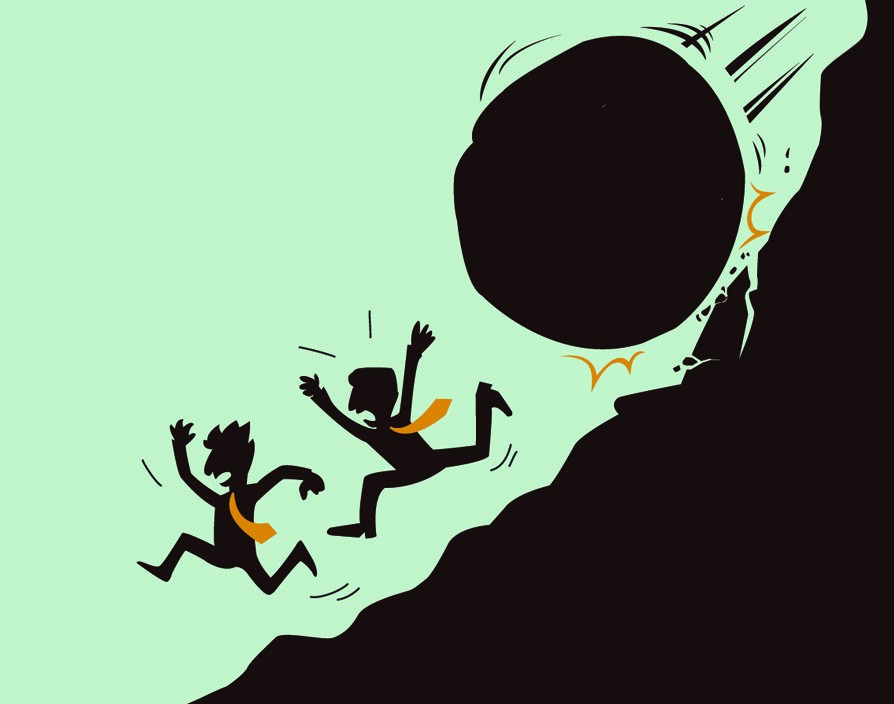
\includegraphics[height=0.8\textheight]{crisis-pic} \\
    {\em Jetzt} ist was anderes Wichtig. (Bild von \cite{crisis-pic})
\end{frame}


\begin{frame}[c]{Definition: Unerledigtes}
    \begin{itemize}[<+(1)->]
        \item Antworten, die ausstehen (z.B. Mails)
        \item Angefangene Projekte
        \item Unaufgeräumte Unterhosen
        \item Ungezahlte Steuern (z.B. für Haustiere)
        \item Veranstaltungen, für die man noch etwas Vorbereiten muss (z.B. Todos)
        \item Doktorbesuche, Reparaturen, Termine
        \item Versprechen, die noch zu erledigen sind
    \end{itemize}
    \pause
    Alles, was noch nicht erledigt ist, aber es (bald) sein
    sollte. Sei konkret, 'reich werden' zählt nicht.
\end{frame}



\begin{frame}[c]{Gegenargument: Aber ich merk mir das}
    \pause
    
\includegraphics[height=0.9\textheight]{forgetting}
    (Bild von \cite{forgetting-pic})
\end{frame}


\begin{frame}[c]{Aufgabe: Situation erfassen}
    \Large
    \begin{itemize}[<+(1)->]
        \item Schreib alles auf, was deine Aufmerksam hat (oder haben sollte!)
        \item Sowohl Privat, als auch für's Studium oder die Arbeit!
        \item Erledige alles direkt, was weniger als 2min braucht!
        \item Ziele kommen auf eine separate Liste!
    \end{itemize}
\end{frame}


\begin{frame}[c]{Hilfsmittel}
    \Large
    \begin{itemize}[<+(1)->]
        \item Deine (aktuelle) todo-Liste (und weitere)
        \item Stift \& Papier (oder anderes Listenerstellungswerkzeug)
        \item GTD Mind Sweep Trigger List \cite{trigger-list} ( \url{https://gettingthingsdone.com/wp-content/uploads/2014/10/Mind_Sweep_Trigger_List.pdf} )
    \end{itemize}
\end{frame}


\addtocounter{framenumber}{1}
\begin{frame}[standout]
    Machen (30min)
\end{frame}

\subsection{Organisation}

\begin{frame}[c]{Definition: Projekt}
    Ein \blue{Projekt} ist alles, was \textbf{mehr als eine} \green{konkrete
    Aufgabe} benötigt, um abgeschlossen zu werden. \newline \newline \pause
    \textbf{Beispiel:} Wenn man \blue{jemandem ein Geschenk besorgen}
    will, muss man zuerst \green{herausfinden, was die Person mag.}
\end{frame}


\begin{frame}[c]{Definition: Kontext}
    % locations, people
    \orang{Kontext} beschreibt eine \textbf{konkrete Eigenschaft} einer
    \green{Aufgabe} oder einem \blue{Projekt.} Häufig die Abhängigkeit zu einem
    bestimmten \textbf{Ort}, einer \textbf{Umgebung}, oder \textbf{Person}.
    \newline \newline \pause
    \textbf{Beispiele:}
    \begin{itemize}[<+(1)->]
        \item \orang{Zuhause}, \orang{am PC}
        \item \orang{dauert kurz}, \orang{dauert lang}
        \item \orang{treffen Mentor}, \orang{treffen Tobi}
    \end{itemize}
\end{frame}


\begin{frame}[c]{Aufgabe: Projekte zusammenfassen}
    Fasse thematisch zusammenhängende \green{Aufgaben} zu \blue{Projekten} und
    \orang{Kontexten} zusammen, und markiere zusammengehörende Elemente
    eindeutig (z.B.: symbol mit einheitlicher Farbe).
    
\end{frame}


\begin{frame}[c]{Bemerkungen}
    Normal ist:
    \begin{itemize}[<+(1)->]
        \item Dir fallen weitere Aufgaben ein, die Unerledigt sind ($\rightarrow$ aufschreiben)
        \item Dir fällt auf, dass etwas ein Projekt ist \\ ($\rightarrow$ finde heraus, was die {\em nächste unerledigte Aufgabe} ist)
    \end{itemize}
\end{frame}


\addtocounter{framenumber}{1}
\begin{frame}[standout]
    Machen (20min)
\end{frame}

\begin{frame}[standout]
    Pause (10min)
\end{frame}

\subsection{Rückblick}

\begin{frame}[c]{Optional: Jahresrückblick}
    \begin{itemize}[<+(1)->]
        \item Zusätzliche, ausführliche Trigger-List
        \item Kann {\em sehr} viel Zeit in anspruch nehmen
        \item Kann sinn machen, gleichzeitig Ziele zu sammeln
        \item Ressourcen: \url{https://drive.google.com/file/d/0B2PaeRjVqAN7MngxTXFPQkpLVjg/view} \cite{8760-hours} (p11-15) (oder anschließend in dieser PDF)
    \end{itemize}
\end{frame}

% \includepdf[pages={11-15},frame,pagecommand={},width=\textwidth]{8760-hours-v2.pdf}
% \includepdf[fitpaper=true,pages=-,frame,pagecommand={},width=\textwidth]{8760-hours-v2.pdf}
{
    \addtocounter{framenumber}{5}
    \setbeamercolor{background canvas}{bg=}
    \includepdf[pages={11-15}]{8760-hours-v2.pdf}
}



